\subsection{Löhne}
\subsubsection{Schweiz}
In der Schweiz sind die Lebensgrundkosten sehr hoch, und dafür ist es wichtig dass die Arbeiter angemessen bezahlt werden um zu gewährleisten dass ein gewissen Lebensstandard einzuhalten. Unter dem Motto "Ein glücklicher Mitarbeiter ist ein produktiver Mitarbeiter " werden in der Schweiz gemäss
(„Branchenverband Deutschschweizer Wein“ , 2016) auch anständige Löhne für die hiesigen Mitarbeiter bezahlt. Mit einem Einstiegslohn von rund 4700 werden Winzer auch für die körperlich anstrengende Arbeit gerecht entlohnt. Durch das schweizerische Dreisäulensystem dient als angemessene Sicherung des Existenzbedarf und gilt als Sicherheit für die Arbeiter. Im ganzen gesehen ist der Beruf des Winzers in der Schweiz als sicher zu betrachtet.

\subsubsection{Kalifornien}

Der durchschnittliche Verdienst in den Vereinigten Staaten von Amerika beträgt rund um die 3080 US Dollar pro Monat. (Quelle: Erhebung des US Census) Dieser Betrag schwankt ein wenig von Staat zu Staat, aber dient hier nur als Vergleich. Bezüglich des Verdienstes spielt es in der kalifornischen Weinproduktion eine essenzielle Rolle welchen Beruf ausgeübt wird. So verdient ein sogenannter «Winemaker», was der Chef einer Kellerei ist, um die 9000 US
Dollar und ein Assistent um die 5 730 US Dollar pro Monat. Diese Werte liegen beide ziemlich weit über den weiter oben genannten Nationalen Durchschnitt. Zu beachten gilt hier dass nur wenige Personen diese Berufung pro Kellerei ausüben. Der Grossteil der Arbeit
wird von sogenannten «grape picker» verrichtet. Diese Pflücken die Weintrauben auf dem Feld. Ein solcher Feldarbeiter verdient im Durchschnitt circa 10 US Dollar pro Stunde,
\cite{_farm_????} hochgerechnet auf ein pro Monat macht das 1500 US Dollar, dies ist um einiges weniger als der Durchschnitt. Die harte Feldarbeit wird zu einem grossen Teil von mexikanischen Immigranten verrichtet, ähnlich in Spanien bei welchen die Feldarbeit von polnischen Immigranten verrichtet wird.
  \begin{figure}[H]
	\centering
	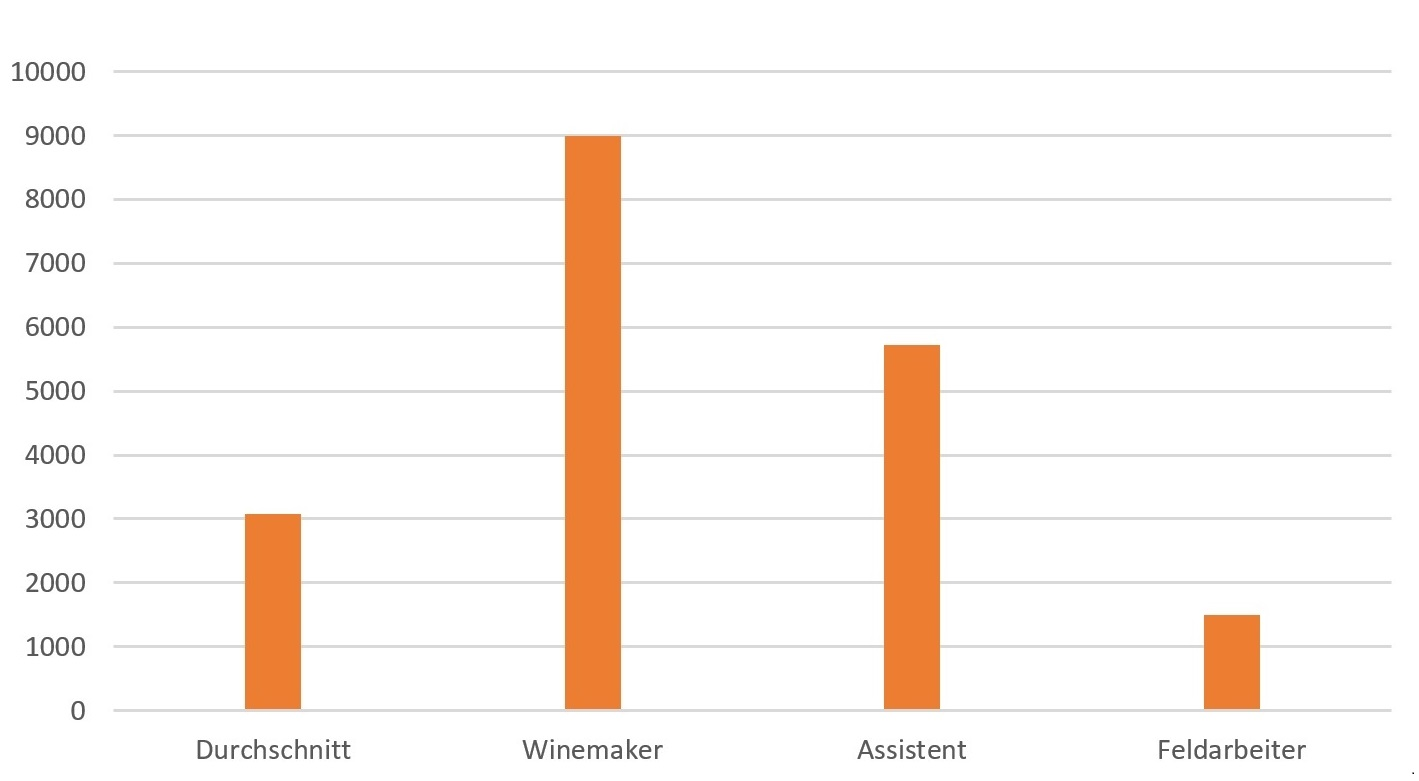
\includegraphics[width=0.9\textwidth]{Grafikarbeiter}
	\caption{Löhne der Arbeiter in der Weinproduktion}
\end{figure}
Die Arbeitsbedingungen in der USA sind im Verhältnis zur Schweiz rückständig, so hat ein Arbeitnehmer in den USA praktisch keinen Kündigungsschutz. Dies liegt an der grossen Mobilität an den Amerikanern. Die amerikanischen haben aber Anspruch auf eine Rente, welche sie ähnlich der Schweiz mit ihrem Lohn bezahlen. \cite{_arbeitszeiten_????} Wie man unschwer erkennt ist das ein Feldarbeiter in Kalifornien unterbezahlt. Hier liegt auch ein grosses Verbesserungspotenzial. Ein gerechter MIndestlohn der per Gesetz geregelt ist, ähnlich wie in der Schweiz, würde die Lage für viele der Feldarbeiter stark verbessern. Du beachten ist dass ein Feldarbeiter im Schnitt nur ein Monat auf den Feldern arbeitet, so ist eher eine Temporäre Anstellung und eine Gesetzgebung könnte sich als schwer gestalten, denn je nach Ernte und Jahr  müssen die Winzer flexibel reagieren können.




